%% Koma Script ------------------------------------------------------------
\documentclass[%
   11pt,              % Fontsize
   english,           % Language
   a4paper,           % Paper Size
   DIV11,             % Print Space / Type Area
   BCOR12mm,		  % Binding Correction
   titlepage,		  % Titlepage
   bibtotoc,		  % Insert Bibliography to ToC
   liststotoc,		  % Insert Listings to ToC
   final,			  % final | draft
   twoside,			  % twosided document
   openright,		  % begin sections on the right side
   cleardoubleempty   % no double empty pages
]{scrreprt}%     Alternatives: scrartcl, scrreprt, scrbook
% -------------------------------------------------------------------------

\usepackage[utf8]{inputenc}
\usepackage{babel}
\usepackage[T1]{fontenc}
\usepackage{textcomp}
\usepackage{lmodern}
\usepackage{graphicx}
\usepackage{tabularx}
\usepackage{hyperref}

% Pagemarks / Headlines
\usepackage{scrpage2}
\pagestyle{scrheadings}
\clearscrheadfoot
\automark[section]{chapter}
\setheadsepline{.4pt}
\ihead[]{\leftmark}
\ohead[]{\rightmark}
\ofoot[\pagemark]{\pagemark}


%%%%%%%%%%%%%%%%%%%%%%%%%%%%%%%%%%%%%%%%%%%%%%%%%%%%%%%%%%
\begin{document}

% Title- and Prefixpages
\begin{titlepage}
 \input{titlepage.inc}
\end{titlepage}

% Create Table of Contents
\tableofcontents

\chapter{Introduction}

\chapter{Architecture}
% Event Driven Design
% Class Diagram Core
% Plugin Concept
% Class Diagram Plugin Wiimote
% Class Diagram Plugin Android


\chapter{Requirements}
The core of wiigee, wiigee-lib, is written device independent and therefore does not have any additional requirements beside of Java\footnote{Sun's Java Website: \url{http://java.sun.com/}, last access \today} in a version greater or equal to 1.6. wiigee-lib only needs acceleration data and discrete events to control the training and recognition process. Both, acceleration and discrete events like e.g. button presses, can be either simulated or generated online by any device. In general every device capable of sending these information is supported by wiigee-lib. A developer only has to make sure that the device can be connected and the corresponding data can be obtained. As the name 'wiigee' already suggests, wiigee-lib has been developed for Nintendos Wii Remote, which is usually named Wiimote.

\section{Wiimote: \texttt{wiigee-plugin-wiimote}}
Nintendos Wiimote usually comes with the popular gaming console Wii, but can also be obtained separately for about \$35 (valid on July, 31th 2009). As required by wiigee-lib, the Wiimote serves acceleration data with a frequency of $100Hz$ and discrete events in form of button presses. The Wiimote serves this data using Bluetooth. Of course Nintendo did not release any information about how to connect to the Wiimote. Every information about the communication protocol has been reverse engineered\footnote{Wiibrew: \url{http://www.wiibrew.org/}, last access \today}. The wiigee-plugin-wiimote implements a part of this reverse engineered information to obtain acceleration and button data from the Wiimote.

\subsection{Bluetooth Device}
As already mentioned the Wiimote uses Bluetooth. Therefore your device where the wiigee-lib is running on needs a Bluetooth dongle or an internal Bluetooth chip. To reach a good data throughput, especially with the frequent acceleration events, consider to get a Bluetooth 2.0 dongle with enhanced data rate (EDR).

\subsection{Bluetooth Stack}
The most important thing for wiigee is the used Bluetooth stack. This is the software, which actually controls your Bluetooth device. Common stacks on Windows are WIDCOMM\footnote{Broadcomm Website: \url{http://www.broadcom.com/}, last access \today}, BlueSoleil\footnote{Bluesoleil Website: \url{http://www.bluesoleil.com/}, last access \today} and the default Windows Bluetooth stack. Linux computers usually uses the BlueZ\footnote{BlueZ Website: \url{http://www.bluez.org/}, last access \today} Bluetooth stack. Apple's OS X already comes with an integrated Bluetooth stack.

\subsection{JSR-82 Implementation}
The JSR-82 implementation actually lets Java know what Bluetooth is and for example how to create connections. Originally specified by a consortium of multiple device manufacturers, there now exists multiple different JSR-82 implementations, like e.g. BlueCove\footnote{BlueCove Website: \url{http://www.bluecove.org/}, last access \today} or Avetana\footnote{Avetana Website: \url{http://www.avetana-gmbh.de/avetana-gmbh/jsr82.xml}, last access \today}. Since the Wiimote uses a specific Bluetooth subprotocol it is necessary that the JSR-82 implementation supports L2CAP for the used Bluetooth stack.

\subsection{Recommendations}
Ok, among us there are not too many working configurations. If you still have the possibility to choose your Bluetooth device consider to buy one which comes with the WIDCOMM Bluetooth stack. This would help you to get wiigee-plugin-wiimote working on Windows. On Linux or OS X systems you could buy any compatible stack. By experience I would recommend the BlueCove JSR-82 implementation, which worked very well for me already on WIDCOMM, BlueZ and the OS X stack.

\section{Android Phone: \texttt{wiigee-plugin-android}}
While the wiimote is a separate device and wiigee's logic runs on a computer, wiigee can also run on a platform equipped with an accelerometer itself. Google's Android is such a Java-enabled platform which wiigee out-of-the-box supports. Any other mobile phones with Java and Accelerationsensor can be adopted easily. Since the Android Developers changed something within the API the wiigee-plugin-android is only working on Android Devices with a firmware greater or equal to Android 1.5.


\chapter{Integrating wiigee into a Java Project}
Integrating wiigee into your Java project is easy. After wiigee's JAR file and at least one plugin has been integrated into the classpath, a \texttt{GestureListener} has to be setup being responsible for received gestures within your application. The following lines describe, how wiigee can be integrated using the well known Netbeans IDE\footnote{Netbeans Website: \url{http://www.netbeans.org/}, last access \today}. Obviously first of all a copy of wiigee is needed, which contains of \textit{wiigee-lib-1.5.6.jar} and in case of the Wiimote complemented by \textit{wiigee-plugin-wiimote-1.5.6.jar}. As already mentioned, a JSR-82 implementation is needed: BlueCove for example \textit{bluecove-2.1.0.jar}.

\section{Netbeans 6.7}

\subsection{Create a new Java Project}
Choose \textbf{File} and select \textbf{New Project}. Then select that a \textbf{Java Application} should be created and click \textbf{Next}.

\begin{figure}[h]
\centering
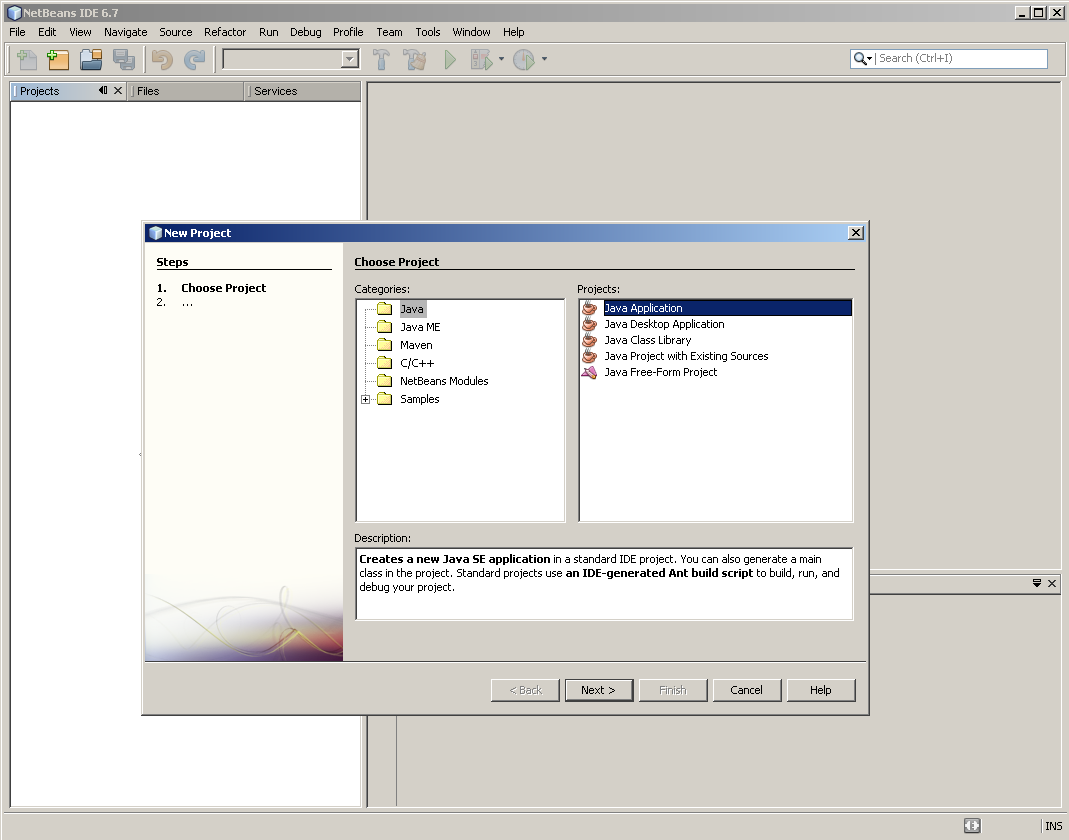
\includegraphics[width=0.95\linewidth]{img/setup/netbeans/step1.png}
\end{figure}

Choose a \textbf{Project Name} like "`wiigee-test"', select \textbf{Use Dedicated Folder for Storing Libraries} and click \textbf{Finish}. Remember the folder where you create your new project.

\begin{figure}[h]
\centering
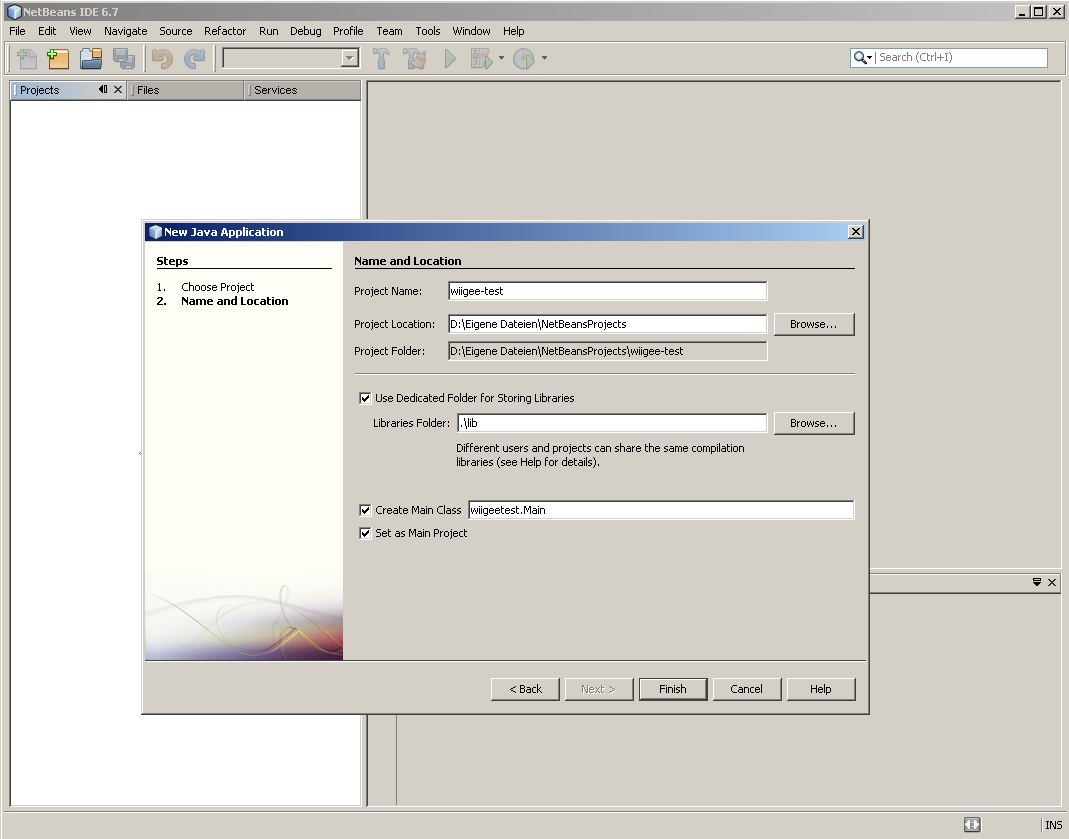
\includegraphics[width=0.95\linewidth]{img/setup/netbeans/step2.png}
\end{figure}

\subsection{Integrate wiigee}
Right click on your project name on the left and select \textbf{Properties}. Then select \textbf{Libraries} and click \textbf{Add JAR/Folder}, since multiple JAR files should be added.

\begin{figure}[h]
\centering
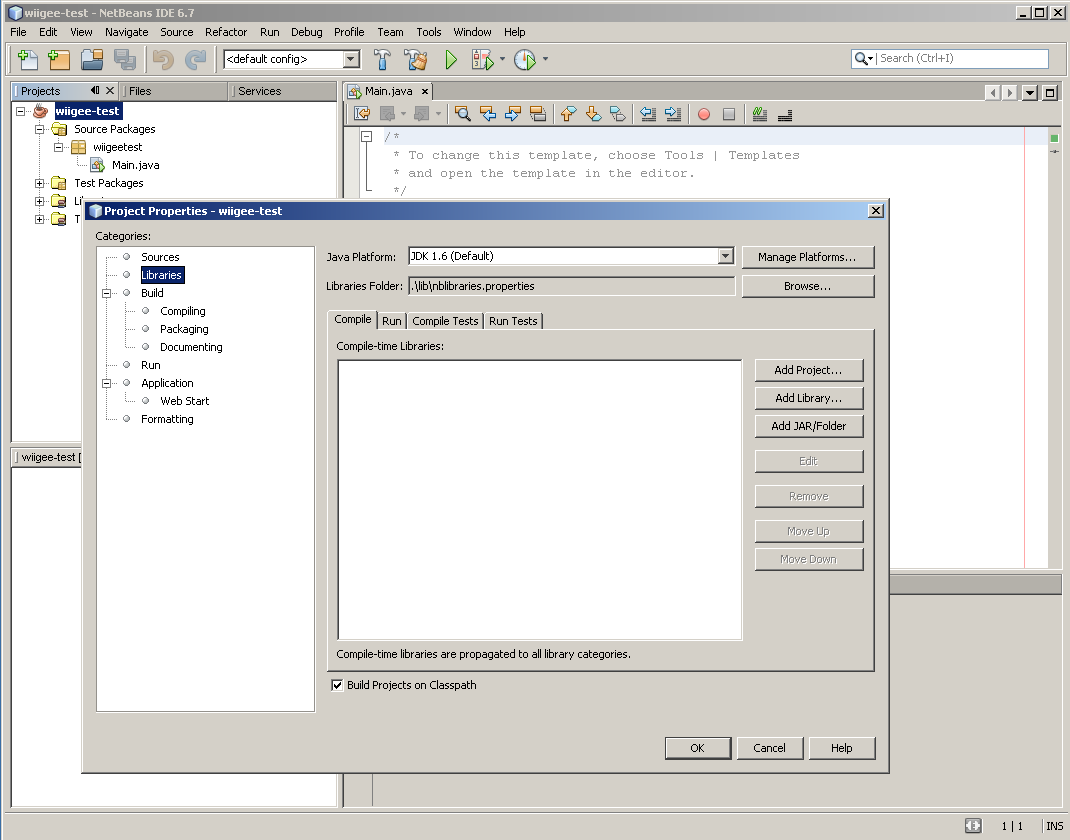
\includegraphics[width=0.95\linewidth]{img/setup/netbeans/step3.png}
\end{figure}

In the popping up file selector, \textbf{change to the path} where you've downloaded wiigee, a wiigee plugin and your JSR 82 implementation. \textbf{Select} the JAR file and select \textbf{Copy to Libraries Folder}. This allows you to delete the downloaded files afterwards, since a copy of them now exists within your project folder. Finally click \textbf{Open}. Repeat this procedure for every JAR file or select multiple libraries at once.

\begin{figure}[h]
\centering
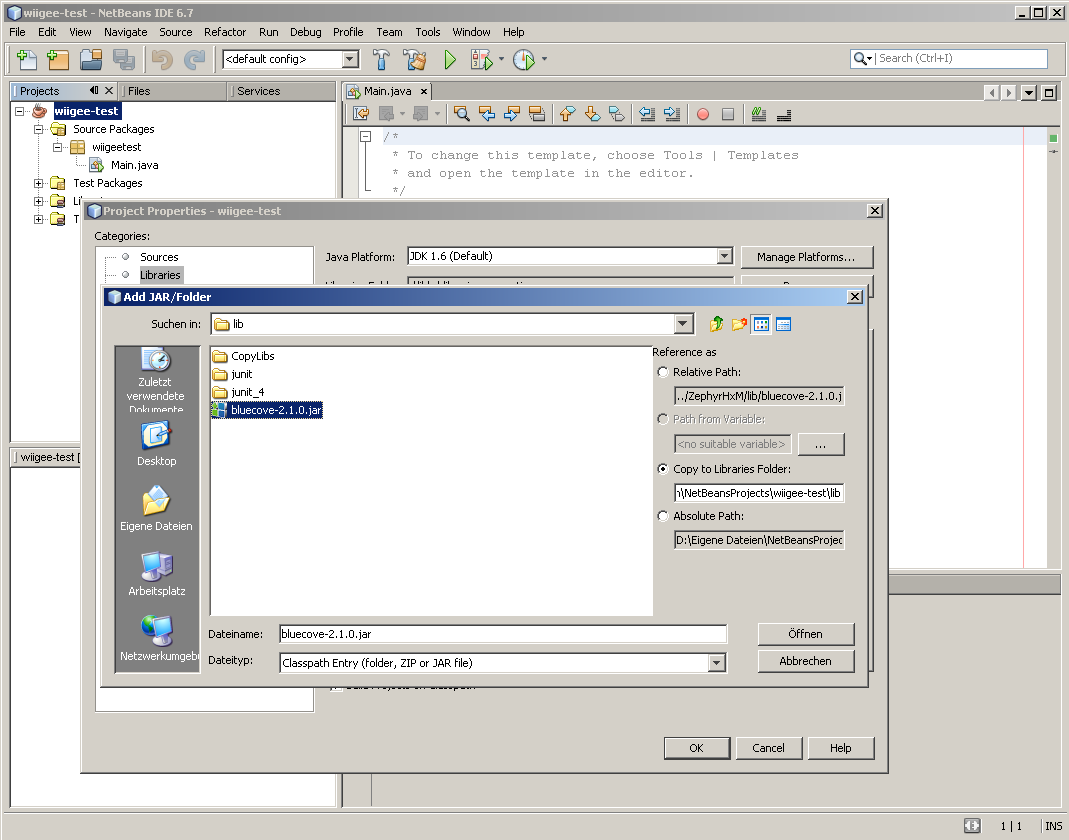
\includegraphics[width=0.95\linewidth]{img/setup/netbeans/step4.png}
\end{figure}



\subsection{Implement GestureListener}
\subsection{Run Application}


\section{Eclipse 3.X}


\chapter{Using wiigee}
\section{Settings}
\subsection{Button Events}

\subsection{Acceleration}
% Filter

\subsection{Rotation}
% Filter

\subsection{Infrared}
% Mouse Control

\chapter{Example: Gesture Controlled Photo Slideshow}
Lorem ipsum dolor sit amet, consectetuer adipiscing elit, sed diam nonummy nibh euismod tincidunt ut laoreet dolore magna aliquam erat volutpat. Ut wisi enim ad minim veniam, quis nostrud exerci tation ullamcorper suscipit lobortis nisl ut aliquip ex ea commodo consequat. Duis autem vel eum iriure dolor in hendrerit in vulputate velit esse molestie consequat, vel illum dolore eu feugiat nulla facilisis at vero et accumsan et iusto odio dignissim qui blandit praesent luptatum zzril delenit augue duis dolore te feugait nulla facilisi. Lorem ipsum dolor sit amet, consectetuer adipiscing elit, sed diam nonummy nibh euismod tincidunt ut laoreet dolore magna aliquam erat volutpat. Ut wisi enim ad minim veniam, quis nostrud exerci tation ullamcorper suscipit lobortis nisl ut aliquip ex ea commodo consequat. Duis autem vel eum iriure dolor in hendrerit in vulputate velit esse molestie consequat, vel illum dolore eu feugiat nulla facilisis at vero et accumsan et iusto odio dignissim qui blandit praesent luptatum zzril delenit augue duis dolore te feugait nulla facilisi. Nam liber tempor cum soluta nobis eleifend option congue nihil imperdiet doming id quod mazim placerat facer possim assum.


% Abbildungsverzeichnis
\listoffigures
% Tabellenverzeichnis
\listoftables

%%%%%%%%%%%%%%%%%%%%%%%%%%%%%%%%%%%%%%%%%%%%%%%%%%%%%%%%%%%%
\end{document}
